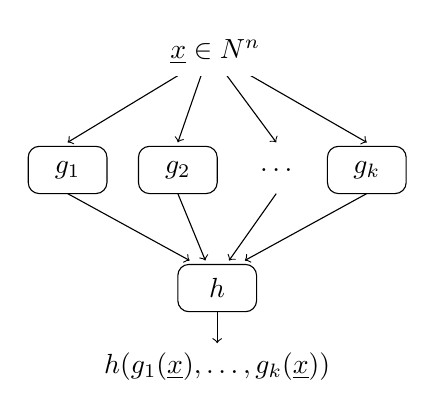
\begin{tikzpicture}
    
    \draw[->]   (0,3)--(-1.9,1.85);
    \draw[->] (-.1,3)--(-.5,1.85);
    \draw[->] (-.1,3)--(.75,1.85);
    \draw[->] (-.1,3)--(1.9,1.85);
    \draw (-2.4,1.2)[rounded corners] rectangle (-1.4,1.8)
        node[midway] {$g_1$};
    \draw (-1,1.2)[rounded corners] rectangle (0,1.8)
        node[midway]  {$g_2$};
    \node at(0.75,1.5) {$\dots$};
    \draw (1.4,1.2)[rounded corners]  rectangle (2.4,1.8) node[midway]  {$g_k$};
    
    \draw (-.53,2.7)[fill=white,white] rectangle (.48,3.3)
        node[midway,black] {$\underline{x} \in \mathbb{N}^n$};
    \draw (-.5,-.3)[rounded corners,fill=white] rectangle (.5,.3) node[midway] {$h$};

    \draw[->] (-1.9,1.2)--(-.35,.35);
    \draw[->] (-.5,1.2)-- (-.15,.35);
    \draw[->] (.75,1.2)-- (.15, .35);
    \draw[->] (1.9,1.2)-- (.35, .35);
    \draw[->] (0,-.3)--(0,-.7);
    \node at(0,-1) {$h(g_1(\underline{x}),\dots,g_k(\underline{x}))$};

\end{tikzpicture}
